\chapter{Annexes de la partie 1}\label{annexe-1}
\dochaptoc

\section{Choix entre la matrice de covariance et matrice de corrélation pour le calcul de l'ACP}\label{abstr-pca-corr-cov}

        Lors du calcul de l'ACP, l'opérateur doit choisir quelle matrice analyser spectralement : la matrice de covariance ou la matrice de corrélation. Le défaut de la matrice de covariance est que les composantes principales sont \guillemets{tirées} en direction des variables dont la variance est la plus forte tandis que la matrice de corrélation capture un nombre important de composantes mineures dont certaines peuvent être aparentées au bruit.

        Nous utilisons le spectre-image $\mathsf{R}_2$ présenté à la \cref{sec-donnees-hr} afin de visualiser ces effets et de choisir quelle matrice utiliser dans nos études.
        %
        Le spectre moyen ainsi que l'évolution de l'écart-type associé à chaque canal sont d'abord affichés à la \cref{fig-pca-variance-data}.
        \begin{figure}
            \centering
            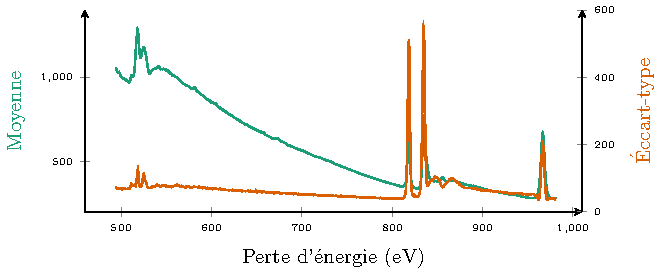
\includegraphics{img/chapitre1/figure16/data_variance.pdf}
            \caption{Le spectre moyen (en vert) et l'éccart-type associé aux canaux (en orange) sont affichés pour le spectre-image $\mathsf{R}_2$ présenté à la \cref{sec-donnees-hr}.
                \protect\label{fig-pca-variance-data}}
        \end{figure}
        On observe entre autre une divergence assez importante entre les écarts-types correspondants aux premiers seuils et ceux associés aux deux seuils centraux. En particulier, les pics dont la variance est la plus importante correspond à des signatures caractéristiques d'éléments présents en abondance à certaines positions et absents à d'autres. Les seuils de variances plus faibles correspondent, au contraire, à des éléments présents en petite quantité sur l'ensemble de l'échantillon. \`A la vue de cet écart de variance, on peut s'attendre à une différence marquée entre les composantes principales issues des deux matrices de covariance et de corrélation. Pour confirmer cela, les cinq premières composantes principales issues des matrices de covariance et de corrélation sont affichées à la \cref{fig-pca-comps_matrices}.
        \begin{figure}[t]
            \centering
            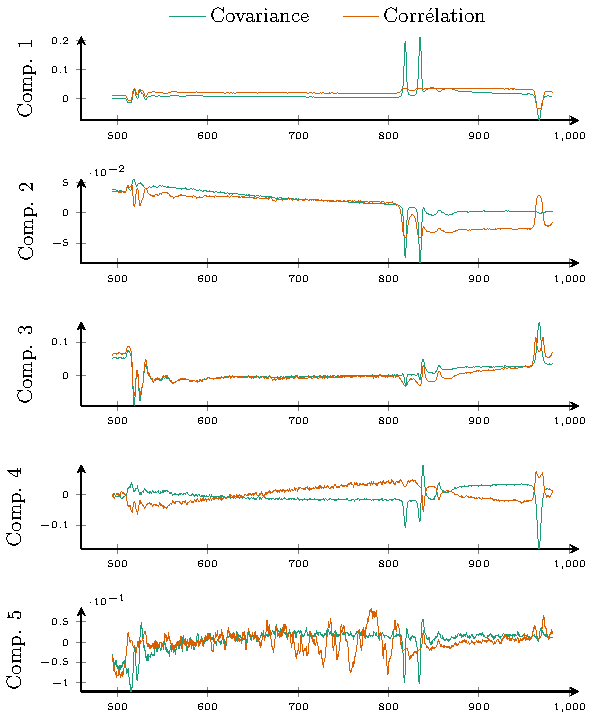
\includegraphics{img/chapitre1/figure16/centerd_spectra_comp.pdf}
            \caption{Représentation des composantes principales estimées à l'aide de la matrice de covariance (en vert) et de corrélation (en orange).
                \protect\label{fig-pca-comps_matrices}}
        \end{figure}
        De plus, les proportions de la puissance totale associées à chaque composante principale pour les deux choix de matrices sont données à la \tabname~\ref{tab-pca-comps_percentage}
        \begin{table}
            \centering
            \begin{tabular}{cccccc}
                \toprule
                Composante&1&2&3&4&5\\
                \midrule
                Covariance & 60.7 & 9.64 & 1.60 & 0.618 & 0.161\\
                Corrélation& 35.2 & 10.7 & 1.92 & 0.626 & 0.208\\
                \bottomrule
            \end{tabular}
        \vspace{1em}
        \caption{Proportion de la puissance en pourcentage pour les cinq premières composantes principales et pour les deux types de matrices.
                \protect\label{tab-pca-comps_percentage}}
        \end{table}

        En considérant les spectres, l'on observe que le premier spectre associé à la matrice de covariance ne regroupe que les seuils de variance supérieure (les deux pics centraux et le dernier pic) tandis que le seuil situé vers \np[eV]{550} est d'amplitude réduite. La deuxième composante capture un fond décroissant, mais seule la paire de pics est capturée. Il faut attendre les composantes 3 et 4 afin de capturer des pics de variance moindre. Enfin, la composante 5 présente des variations mineures et de hautes fréquences dues au bruit. A contrario, les spectres associés à la matrice de corrélation ne capturent pas uniquement les seuils les plus puissants, mais également un nombre important de petites variations, rendant compliqué l'interprétation.
        %
        Ainsi, les résultats issus de la matrice de covariance sont bel et bien \guillemets{aimantés} par les seuils de variance supérieure tandis que les spectres issus de la matrice de corrélation présentent davantage de seuils mineurs, voir de bruit pour les dernières composantes. Utiliser la matrice de corrélation permet donc de mettre en évidence que certains pics participent de manière modérée dans certaines signatures spectrales (il s'agit de seuils associés à de faibles structures spatiales), mais elle risque également de capturer des motifs parasites correspondant au bruit.

        De plus, la proportion de la puissance totale reflète la variance des pics capturés. En effet, la première composante de la matrice de covariance compte pour 60\% de la puissance totale puisqu'elle capture uniquement les seuils de variance élevée. Au contraire, celle issue de la matrice de corrélation ne compte que pour 35\% de la puissance totale puisqu'elle capture principalement des seuils de variance réduite, mais les rapports suivants sont tous supérieurs par rapport à la matrice de covariance.

        Finalement, le choix de la matrice à utiliser dépend de la composante à étudier.
        \begin{itemize}
            \item Si l'on s'intéresse à un élément dont l'abondance est très variable, alors la variance associée à ses seuils sera élevée et ceux-ci seront capturés efficacement par l'\gls{acp} si la matrice de covariance est utilisée. C'est notamment le cas pour les images à échelle atomique lorsque l'on s'intéresse à la signature associée à un atome présent en abondance dans une partie importante de l'image. La contrepartie est que les seuils plus mineurs ne seront que peu conservés.
            \item Si l'on s'intéresse à un élément peu abondant et localisé, sa variance sera faible et les seuils associés seront bien mieux conservés en utilisant la matrice de corrélation. Ainsi, les structures fines aux interfaces seront mieux restituées avec cette matrice. Le défaut, c'est que certaines structures parasites pourraient également apparaître à cause du bruit capturé par l'ACP.
        \end{itemize}
        Dans cette étude, la matrice de covariance a été utilisé puisque les éléments étudiés étaient suffisamment abondants.
        
            \section{Diagrammes de Voronoi et triangulation de Delaunay}\label{abstr-voronoi-delaunay}
        
        \begin{marginfigure}
            \centering
            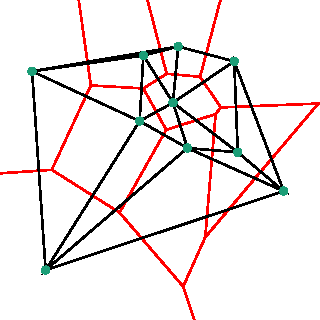
\includegraphics[]{img/chapitre2/figure3/Voronoi.pdf}
            \caption{Superposition d'un diagramme de Voronoi (en rouge) et de sa triangulation de Delaunay (en noir). Le nuage de points est en vert.}
            \label{fig-voronoi}
        \end{marginfigure}
        Les techniques d'interpolation introduites à la \cref{sec-interpolation} requirent deux outils mathématiques simples et complémentaires. Le premier, appelé diagramme de Voronoi~\cite{cazals2006delaunay}, est défini pour un ensemble de points comme suit.
        \begin{mydef}[Diagramme de Voronoi]
            Soit $\mathbb{R}^n$ muni de la distance euclidienne $d$ et $(s_k)_{1\leq k\leq K}$ un ensemble de $K$ points de $\mathbb{R}^n$. La cellule de Voronoi $R_k$ associée au point $s_k$ est l'ensemble des points de $\mathbb{R}^n$ plus proches de $s_k$ que de tout autre point $s_j$ pour $j$ différent de $k$. En d'autres termes, si $d(s_k, s_j)$ désigne la distance entre $s_k$ et $s_j$, nous avons
            \[R_k=\{x\in X | d(x, s_k) \leq d(x, s_j) \ \forall j\neq k\}.\]
            Le diagramme de Voronoi est défini comme l'ensemble des cellules $(R_k)_{1\leq k\leq K}$.
        \end{mydef}
        Le diagramme de Voronoi se visualise bien si la dimension $n$ vaut 2 et cette notion est illustrée en rouge à la~\cref{fig-voronoi}. Une problématique communément associée à ce graphe est la \emph{triangulation} qui consiste à découper un plan en une collection de triangles. En effet, la triangulation de Delaunay~\cite{cazals2006delaunay} d'un ensemble discret de points est le graphe dual du diagramme de Voronoi et se définit comme suit.
        \begin{mydef}[Triangulation de Delaunay]
            Soit $\mathcal{S}=(s_k)_{1\leq k\leq K}$ un ensemble de points appartenant à $\mathbb{R}^n$. Une triangulation de Delaunay $\mathrm{DT}(\mathcal{S})$ est une triangulation telle qu'aucun point de $\mathcal{S}$ ne se trouve dans l'hypersphère circonscrite d'un simplexe de $\mathrm{DT}(\mathcal{S})$.
        \end{mydef}
    \begin{marginfigure}
        \centering
        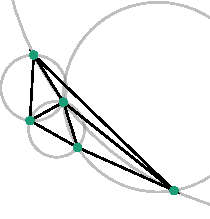
\includegraphics[]{img/chapitre2/figure3/Delaunay.pdf}
        \caption{Superposition d'un ensemble de points (en vert), de sa triangulation de Delaunay (en noir) et des cercles circonscrit à chaque triangle (en gris).}
        \label{fig-delaunay}
    \end{marginfigure}
        Notons qu'une hypersphère circonscrite (resp. un simplexe) est la généralisation du cercle circonscrit (resp. du triangle) en dimension quelconque. La triangulation de Delaunay est illustrée en noir à la \cref{fig-voronoi} et les cercles circonscrit associés à chaque triangle sont mis en évidence pour un ensemble de points réduits à la \cref{fig-delaunay}.